%appendix F
%Gateway Receiver

%\section{Process: Gateway Receiver}

\section{Overview}
\begin{figure}[ht]
    \centering
    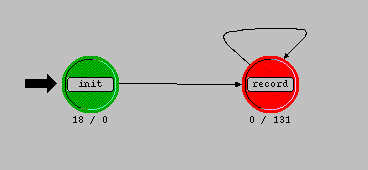
\includegraphics[scale=0.6]{images/gateway_rcvr}
    \caption{Gateway receiver process model}
    \label{fig:appendix-f}
\end{figure}

\newpage
% There are no local variables

\section{Header Block}
%_____________________________________HEADER______________________________________
{\tiny
\begin{verbatim}
#define MAX_SRC_IDS	10
#define IC_SOURCPROP_RX 	99
int has_inited = 0;
int pkt_received[MAX_SRC_IDS*3];
int hack_pkt_keyupnum[MAX_SRC_IDS*3];
Stathandle stat_neworreplace;
Stathandle stat_counterchange;
List *create_stat_lst(char *);

\end{verbatim}
}

\section{Function Block}
%______________________________FUNCTION__________________________________
{\tiny
\begin{verbatim}

List *create_stat_lst(char *statName)
{
	List *lst;
	int stat_size;
	int i;
	FIN(create_stat_lst(char *statName));
	op_stat_dim_size_get (statName, OPC_STAT_GLOBAL, &stat_size);
	if(stat_size != MAX_SRC_IDS)
	{
		op_sim_end("Bad stat dimension", statName, "", "");
	}
	lst = op_prg_list_create();
	for(i = 0; i < MAX_SRC_IDS; i++)
	{
		Stathandle *sth_temp;
		sth_temp = (Stathandle *) op_prg_mem_alloc (sizeof (Stathandle));
		*sth_temp = op_stat_reg (statName, i, OPC_STAT_GLOBAL);
		op_prg_list_insert(lst, sth_temp, OPC_LISTPOS_TAIL);
	}
	FRET(lst);
}

\end{verbatim}
}
\section{init State: Enter Executives}
%______________________________________Init_____________________________________________________________
{\tiny
\begin{verbatim}

int stat_size_temp;
int i;
if(has_inited == 0)
{
	printf("INITIALIZING gateway statistics\n");
	has_inited = 1;
	for(i = 0; i < MAX_SRC_IDS*3; i++)
	{
		pkt_received[i] = 0;
		hack_pkt_keyupnum[i] = -1;
	}
	stat_neworreplace = op_stat_reg("Update Pkt - New or Replace" ,OPC_STAT_INDEX_NONE, OPC_STAT_GLOBAL);
	stat_counterchange = op_stat_reg("Update Counter Change" ,OPC_STAT_INDEX_NONE, OPC_STAT_GLOBAL);
}

\end{verbatim}
}

\section{record State: Exit Executives}
%_____________________________________Record_____________________________________________________________
{\tiny
\begin{verbatim}

Packet *pPkt;
int key;
int sourceid;
int key_updnm;
double generated_timestamp;
int is_update;
int array_index;
Objid source_prop_id;
char message_str [255];

pPkt = op_pk_get(op_intrpt_strm());
if(pPkt == OPC_NIL)
{
	op_sim_end("Nil stream pkt", "", "", "");
}
op_pk_nfd_get(pPkt, "source_id", &sourceid);
op_pk_nfd_get(pPkt, "key", &key);
op_pk_nfd_get(pPkt, "key_update_number", &key_updnm);
op_pk_nfd_get(pPkt, "source_prop_objid", &source_prop_id);
op_pk_nfd_get(pPkt, "generated_timestamp", &generated_timestamp);
//printf("\tEnd getting fields\n");

//Check the fields
if(sourceid < 0 || sourceid >= MAX_SRC_IDS)
{
	op_sim_end("Bad source id", "", "", "");
}
else if(key_updnm < 0)
{
	op_sim_end("Bad key_updnm", "", "", "");
}
else if(key < 1 || key > 3)
{
	op_sim_end("Bad key", "", "", "");
}
array_index = sourceid*3 + (key-1);
is_update = 0;
if(pkt_received[array_index])
{
	int oldkey_updnm = hack_pkt_keyupnum[array_index];
	if(oldkey_updnm < key_updnm)
	{
		is_update = 1;
		op_stat_write(stat_counterchange, key_updnm - oldkey_updnm);
		hack_pkt_keyupnum[array_index] = key_updnm;
	}
}
else
{
	is_update = 1;
	pkt_received[array_index] = 1;
	hack_pkt_keyupnum[array_index] = key_updnm;
}
if(is_update)
{
	Ici *iciptr = op_ici_create ("prop_action");
	op_ici_attr_set (iciptr, "source_id", sourceid);
	op_ici_attr_set (iciptr, "key_update_number", key_updnm);
	op_ici_attr_set (iciptr, "action", 1); //Gateway rx code
	op_ici_attr_set (iciptr, "generated_timestamp", generated_timestamp);
	op_ici_install(iciptr);
	op_intrpt_schedule_remote (op_sim_time (), IC_SOURCPROP_RX, source_prop_id);
	op_stat_write(stat_neworreplace, 1.0);
}
op_pk_destroy(pPkt);


\end{verbatim}
}

